%%%%%%%%%%%%%%%%%%%%%%%%%%%%%%%%%%%%%%%%%%%%%%%%%%%%%%%%%%%%%%%%%
% Tese de Doutorado / Dept. Fisica, CFM, UFSC                   %
% Lacerda@CórregoGrande - Jan/2018                              %
%%%%%%%%%%%%%%%%%%%%%%%%%%%%%%%%%%%%%%%%%%%%%%%%%%%%%%%%%%%%%%%%%

%:::::::::::::::::::::::::::::::::::::::::::::::::::::::::::::::%
%                                                               %
%                 Anexo Laboratório de análises                 %
%                                                               %
%***************************************************************%

\chapter{Laboratório de análises}
\label{apendice:lab}

\section{Pacote de análise da síntese}
 \label{apendice:lab:syntpack}

A confiança na qualidade dos dados observacionais é primordial para o desenvolvimento de qualquer estudo empírico. Nos encarregamos de escrever um pacote de análise da qualidade da síntese de populações estelares com o \starlight, que, em muitos casos, acaba também funcionando como sensor da qualidade dos espectros observados. Esse processo ficou descrito e publicado no artigo de \citet[][DR1]{Husemann.etal.2013a} e foi repetido no DR2 e DR3. Para o último {\em data-release}, essa análise foi feita através de outro grupo dentro do projeto CALIFA, porém, seguindo a linha dos dois primeiros, nós também a produzimos com o \starlight como controle de qualidade dos nossos ajustes espectrais. Comparações com os resultados das amostras anteriores mostram uma importante e gradativa melhora nos espectros resíduais.

%---------------------------- Figure ----------------------------
\begin{figure}
	\centering
	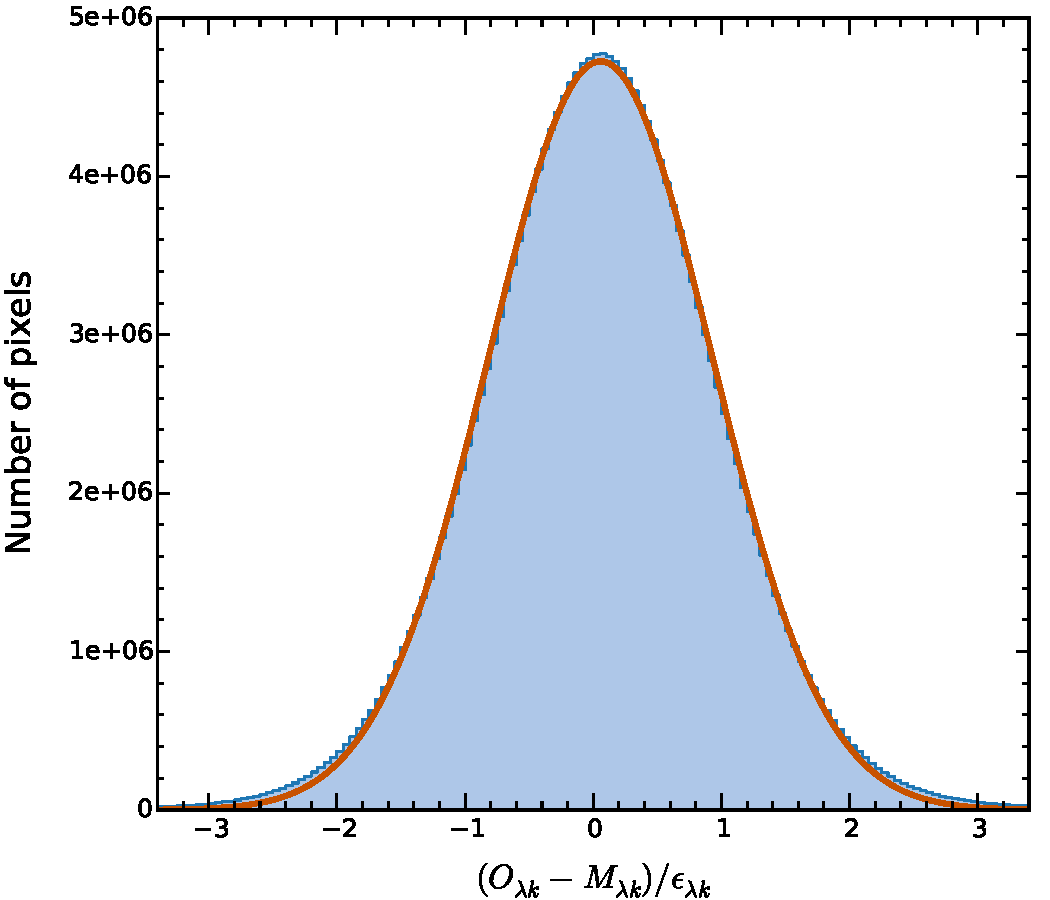
\includegraphics[scale=0.4]{figuras/DR2_hist_error.pdf}
	\caption[Distribuição dos resíduos reduzidos.]
	{Distribuição do resíduo reduzido, $(O_{\lambda,k} - M_{\lambda,k})/\epsilon_{\lambda,k}$, para todos os comprimentos de onda $\lambda$ e todos os espectros $k$ de todas as galáxias presentes no DR2 ($209\,151\,086$ pontos no total). A linha laranja mostra o melhor ajuste Gaussiano para a distribuição (média $= 0.03$; $\sigma = 0.87$). Retirado de \citet{GarciaBenito.etal.2015a}.}
	\label{fig:fres_norm_error_distrib}
\end{figure}
%---------------------------- Figure ----------------------------

A Figura \ref{fig:fres_norm_error_distrib}, que também está publicada no artigo \citet{GarciaBenito.etal.2015a}, põe à prova a qualidade dos ajuste espectrais e também dos erros formais estimados para cada comprimento de onda. Supondo que um espectro residual seja inteiramente formado por ruído, ou seja, modelos estelares e ajustes tão bons quanto se possam ter, sua distribuição deveria ser gaussiana e centrada em zero. Além disso, quando temos um erro formal no fluxo perfeitamente estimado, a distribuição do espectro residual normalizado pelo erro formal no fluxo deveria ser formada basicamente de ruído, por isso, centrada em zero e com $\sigma \sim 1$. Nessa figura vemos o histograma do resíduo reduzido, ou seja, a diferença entre o fluxo observado ($O_{\lambda,k}$) e o modelado ($M_{\lambda,k}$), obtido através da síntese com o \starlight, dividida pelo erro associado ($\epsilon_{\lambda,k}$). Os índices $\lambda$ e $k$ representam um certo comprimento de onda de um certo espectro respectivamente. Dessa análise são excluídos intervalos em $\lambda$ que representam linhas de emissão e dados espúrios. A distribuição é muito bem descrita por uma gaussiana com centro 0.03 e $\sigma = 0.87$, ambos muito próximos dos valores óptimos.

\begin{figure}
	\centering
	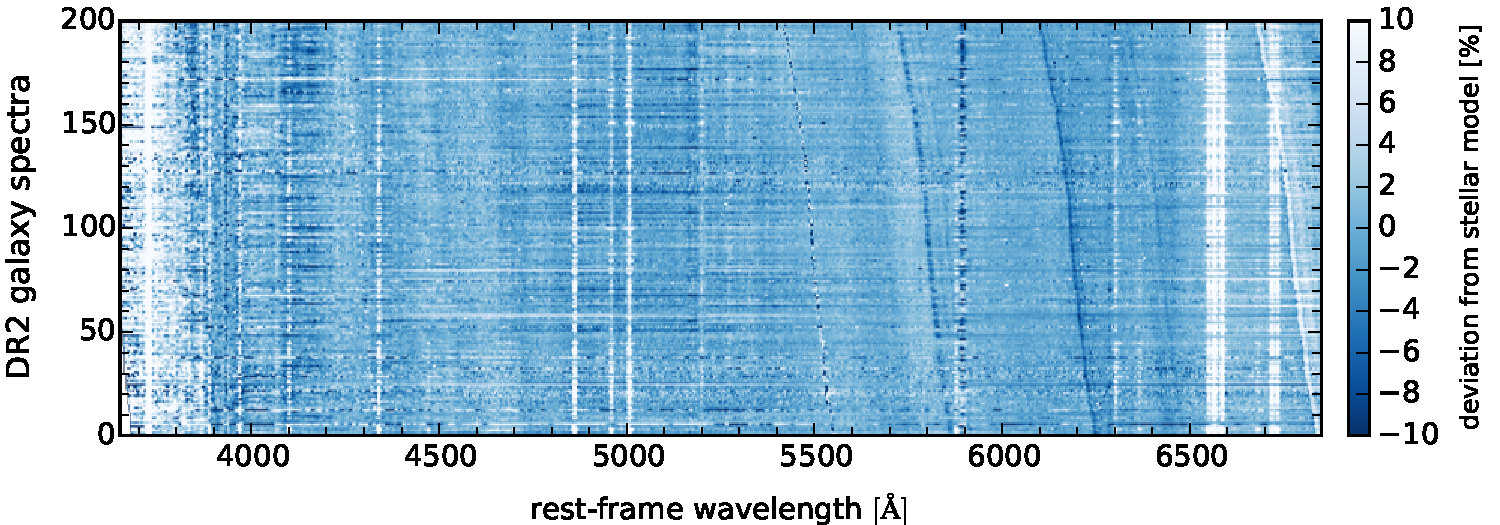
\includegraphics[scale=0.5]{figuras/DR2_stacked_residuals.pdf}
	\caption[Espectros residuais nucleares das galáxias do DR2.]
	{NOMNOMNONMNOMNONM. Retirado de \citet{GarciaBenito.etal.2015a}.}
	\label{fig:fnuc_stack}
\end{figure}

Esta mesma análise nos ajudou a melhorar a máscara de remoção de linhas telúricas\footnote{Linhas provenientes de fenômenos que ocorrem na Terra.} e linhas de emissão dos espectros. A Figura \ref{fig:fnuc_stack} é formada pelos espectros nucleares ajustado para o referencial de laboratóriodas das 200 galáxias presentes no DR2 e ordenados por {\em redshift}. As cores codificam o desvio relativo entre o fluxo observado e o modelado $(O_\lambda - M_\lambda)/O_\lambda$, sem nenhuma máscara espectral.

% End of this chapter
